\section{冗余与纠错}
\label{sec:ccode-redundancy}

第~\ref{chap:discrete-channel-capacity}章的三次重复码把一个比特连发三遍，接收端按多数判决，在$p=0.1$的二元对称信道上把错误概率从$0.1$降到$0.028$。重复的遍数增加时，错误还会怎样变化？具体地说，固定块长$n$以后，多数判决一定能纠正几个翻转？纠不过来的概率又是多少？

\paragraph{多数判决能纠正的翻转数}
取奇数块长$n=2t+1$。消息$0$的码字是$n$个$0$，消息$1$的码字是$n$个$1$。设发送的是全$0$码字，信道翻转了其中$j$个位置，接收块里就有$j$个$1$和$n-j$个$0$。多数判决把它判为$0$，当且仅当$0$占多数，即
\[
 n-j>j,\qquad\text{也就是}\qquad j\leq t .
\]
发送全$1$码字时的情形完全对称。所以长度为$2t+1$的重复码配合多数判决，无论翻转发生在哪些位置，只要不超过$t$个就一定判对；超过$t$个就一定判错。

“一定纠正$t$个”是一个与信道概率无关的组合保证：它只数翻转的个数，不问翻转多常发生。要得到错误概率，还需要知道翻转个数的分布。在二元对称信道上，各位置独立地以概率$p$翻转，所以翻转个数服从$\operatorname{Bin}(n,p)$。判错恰好是翻转个数超过$t$，于是块错误概率为
\begin{equation}
 P_{\mathrm{e}}^{\mathrm{rep}}(n)=\sum_{j=t+1}^{n}\binom{n}{j}p^{j}(1-p)^{n-j},\qquad n=2t+1 .
 \label{eq:ccode-rep-error}
\end{equation}
这里两条消息的错误概率相同，平均错误概率与最大错误概率是同一个数。

\paragraph{块长为五的例子}
取$n=5$，$t=2$，$p=0.1$。至多两个翻转都能纠正，判错需要至少三个翻转。按式~\eqref{eq:ccode-rep-error}逐项计算：
\[
 \begin{aligned}
 \binom53p^3(1-p)^2&=10\times0.001\times0.81=0.0081 ,\\
 \binom54p^4(1-p)&=5\times0.0001\times0.9=0.00045 ,\\
 \binom55p^5&=0.00001 .
 \end{aligned}
\]
三项相加，得到
\[
 P_{\mathrm{e}}^{\mathrm{rep}}(5)=0.00856 .
\]
块长从$3$增加到$5$，错误概率从$0.028$降到约原来的三分之一，码率从$\tfrac13$降到$\tfrac15$。图~\ref{fig:ccode-repetition-flips}(a)画出$\operatorname{Bin}(5,0.1)$的全部质量：蓝色的三根柱是能纠正的情形，合计$0.99144$；红色是判错的情形，几乎看不见，因为三个以上的翻转很少发生。

\begin{BookInlineFigure}
 \centering
 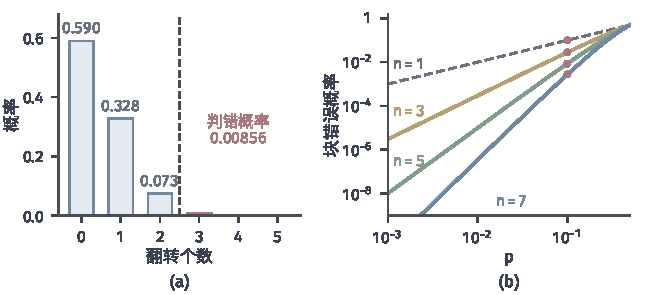
\includegraphics[width=110mm]{figures/07-probability/06-channel-coding/matplotlib/ccode-repetition-flips/figure.pdf}
 \caption{重复码与多数判决。(a) 块长$5$、$p=0.1$时翻转个数的分布$\operatorname{Bin}(5,0.1)$；虚线左侧（蓝）至多两个翻转，一定纠正，右侧（红）一定判错，总概率$0.00856$。(b) 块长$n=1,3,5,7$的块错误概率随翻转概率$p$的变化，双对数坐标；$n=1$（灰色虚线）即不编码，红点标出$p=0.1$处的值。}
 \label{fig:ccode-repetition-flips}
\end{BookInlineFigure}

图~\ref{fig:ccode-repetition-flips}(b)显示了另一面：块长为$2t+1$时，$p$很小的一端曲线的斜率约为$t+1$。原因是式~\eqref{eq:ccode-rep-error}的第一项$\binom{n}{t+1}p^{t+1}(1-p)^{t}$在$p\to0$时起主导作用，错误概率与$p^{t+1}$同阶。能纠正的翻转数$t$决定了噪声变小时错误下降得多快。$p$接近$\tfrac12$时，所有曲线汇合到$\tfrac12$，此时信道输出与输入独立，重复多少遍也没有用。

\paragraph{偶数块长}
块长为偶数时会出现平局。以$n=4$为例，收到两个$0$、两个$1$时，两条消息同样可能，接收端只能任选一个，或者宣布“出错了但不知道是哪条”。所以四次重复码能保证纠正的仍然只有一个翻转，与三次重复码相同，多出来的一次使用只换来了发现两个翻转的能力。区分“发现有错”与“改正错误”，是下一节的主题。

\paragraph{冗余的代价}
重复码的每一份冗余只保护一个消息比特。用三次重复码发送$4$个比特要$12$次信道使用，每个比特独立地以$0.028$的概率出错，$4$位全对的概率是
\[
 (1-0.028)^4\approx0.8926 ,
\]
块错误概率约为$0.107$。不编码时只用$4$次，块错误概率是$1-0.9^4\approx0.344$。三倍的信道使用换来了错误概率的下降，但第~\ref{chap:discrete-channel-capacity}章说明，码率可以接近$0.531$而错误仍趋于零，重复码的$\tfrac13$离此很远。

浪费在哪里？三次重复码把$2^{12}=4096$个可能的接收块分给$16$条消息，平均每条消息占$256$个接收块。但真正需要的只是：每条消息的码字周围，那些“翻转少数几位就能到达”的接收块不要与别的消息混淆。若一个校验位同时参与保护几个消息比特，冗余可以被共享。例如在两个消息比特后面附上它们的模$2$和，任何单个翻转都会让三位之和变成奇数，从而被发现，而码率是$\tfrac23$。只是这一个校验位还不能指出是哪一位出了错。

于是本章面对两个构造问题。一是怎样安排有限的冗余，使不同消息的码字彼此分得足够开，少数翻转之后仍能区分；二是消息很多时，例如$2^{100}$条，怎样不必存储完整的码本，就能完成编码和解码。第~\ref{sec:ccode-min-distance}节用距离回答第一个问题，第~\ref{sec:ccode-linear}节用线性结构回答第二个问题。
